\section{Παρουσίαση αποτελεσμάτων}

\subsection{Προφίλ ταχύτητας στην αξονική θέση του δρομέα}

\begin{figure}[h!]
    \begin{center}
        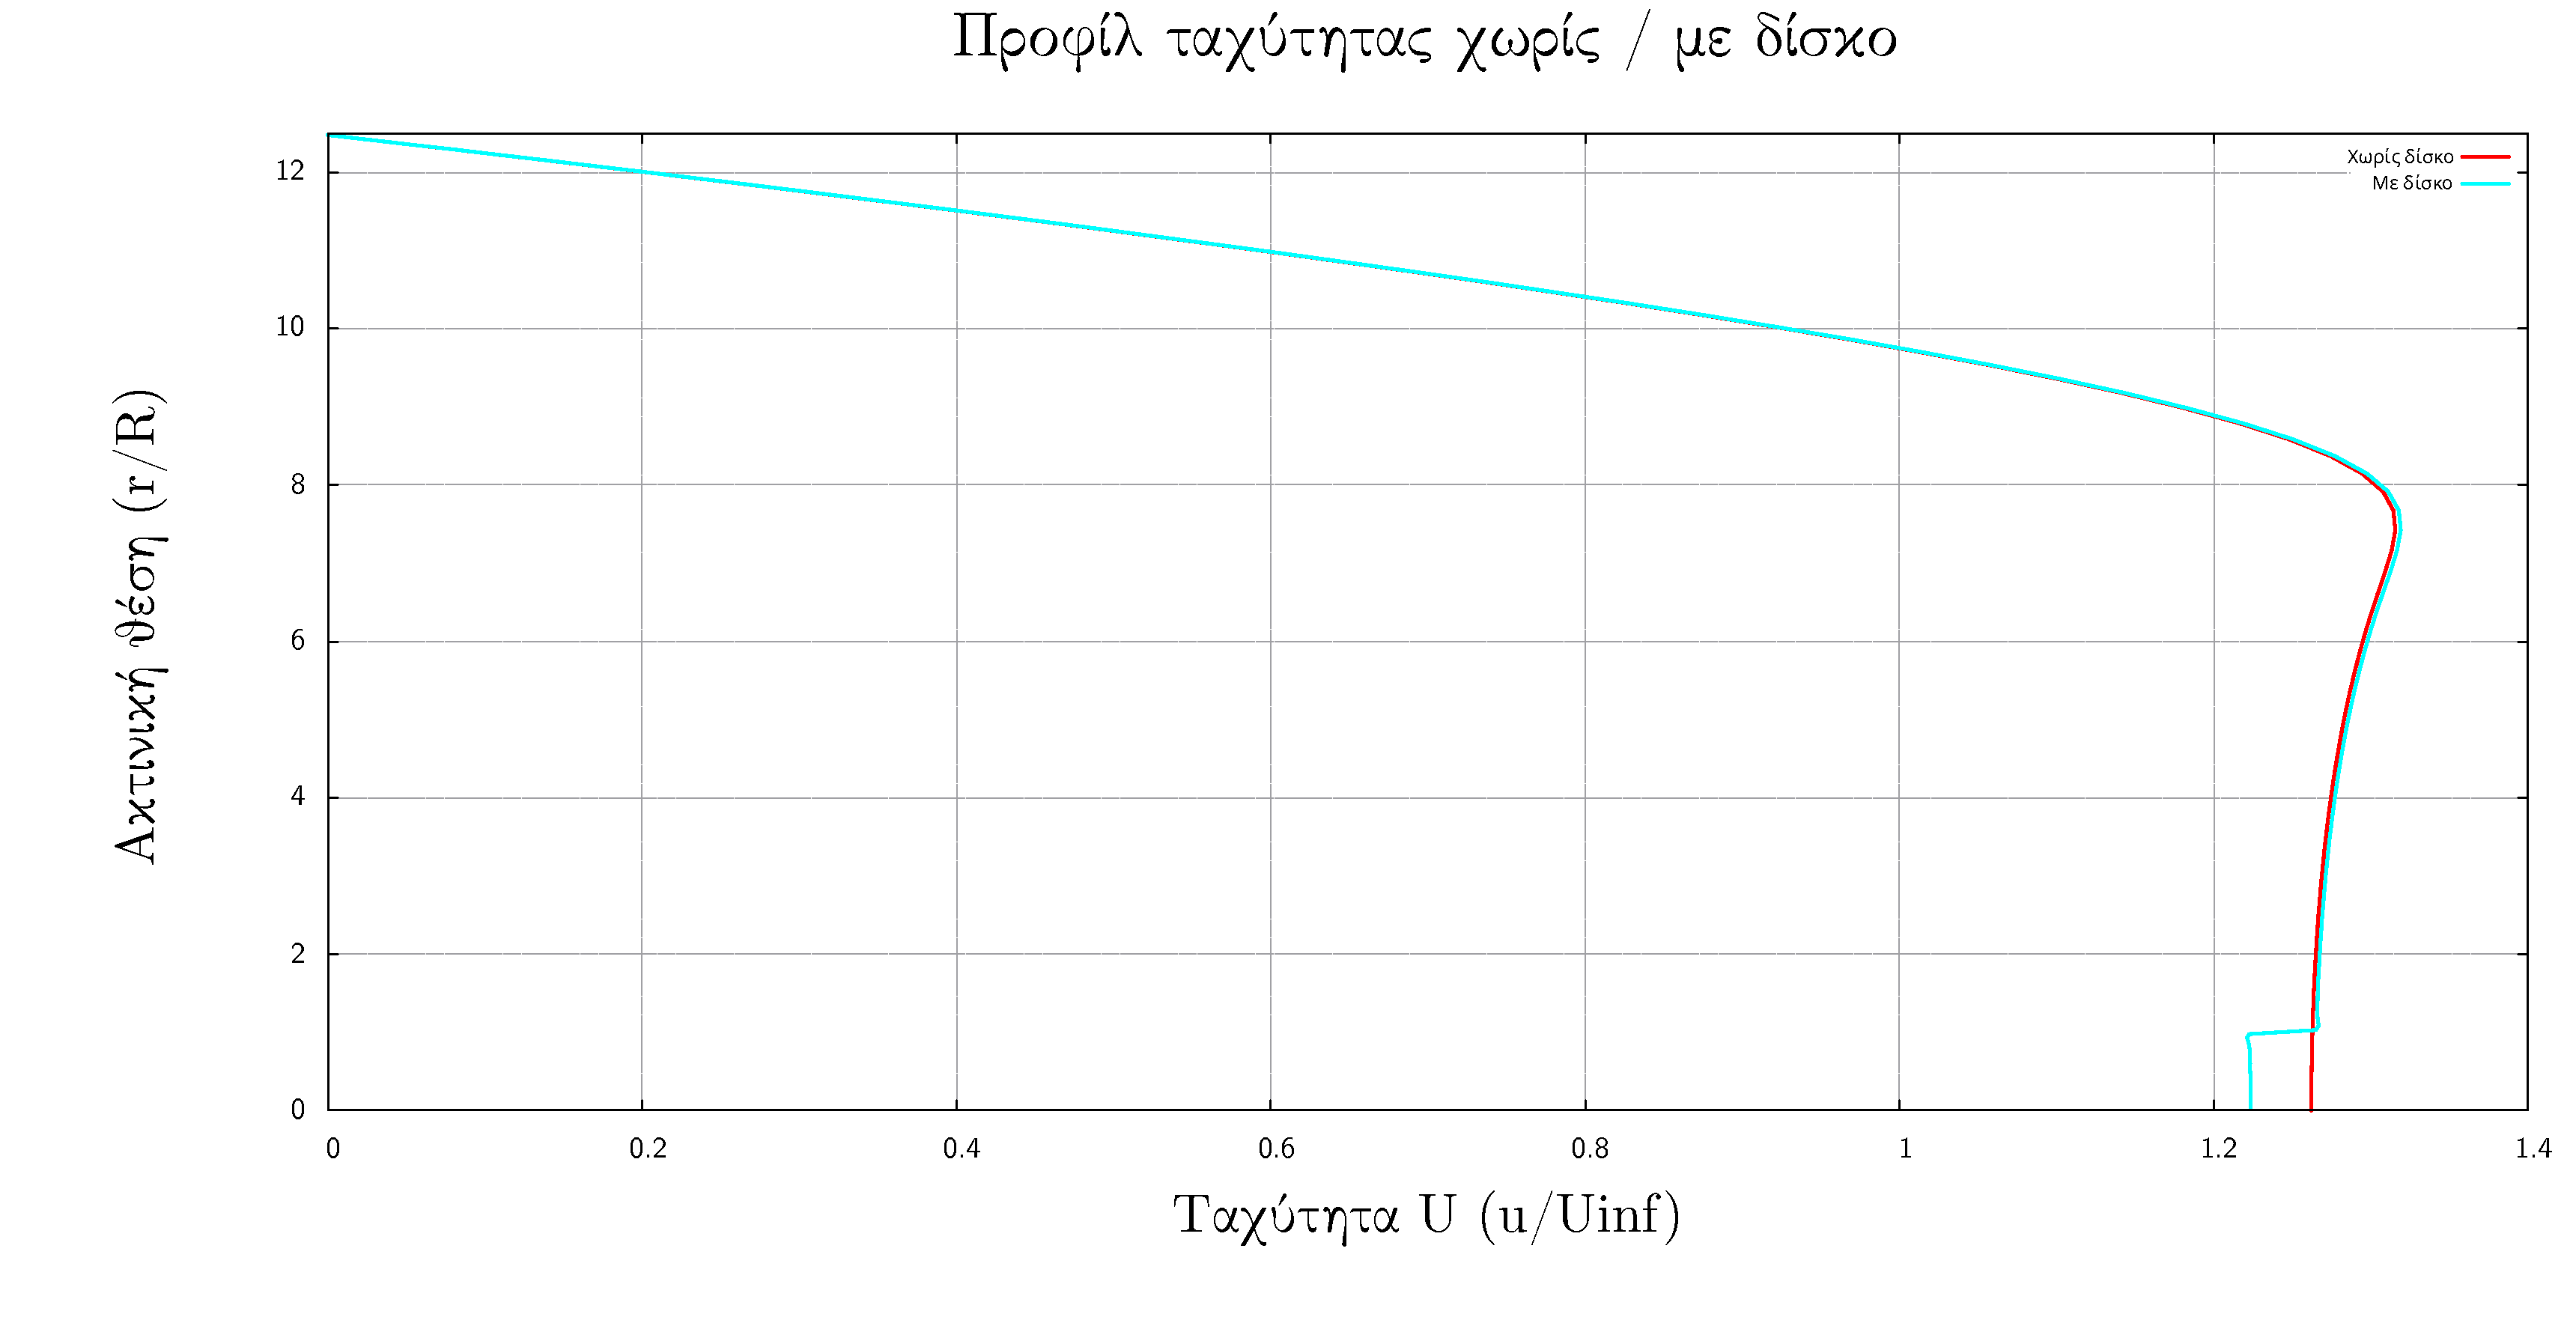
\includegraphics[width=0.75\textwidth]{figures/x0_prof.pdf}
    \end{center}
    \label{fig:x0prof}
\end{figure}

\newpage
\subsection{Ισοταχείς της ροής με δρομέα}

\begin{figure}[h!]
    \begin{center}
        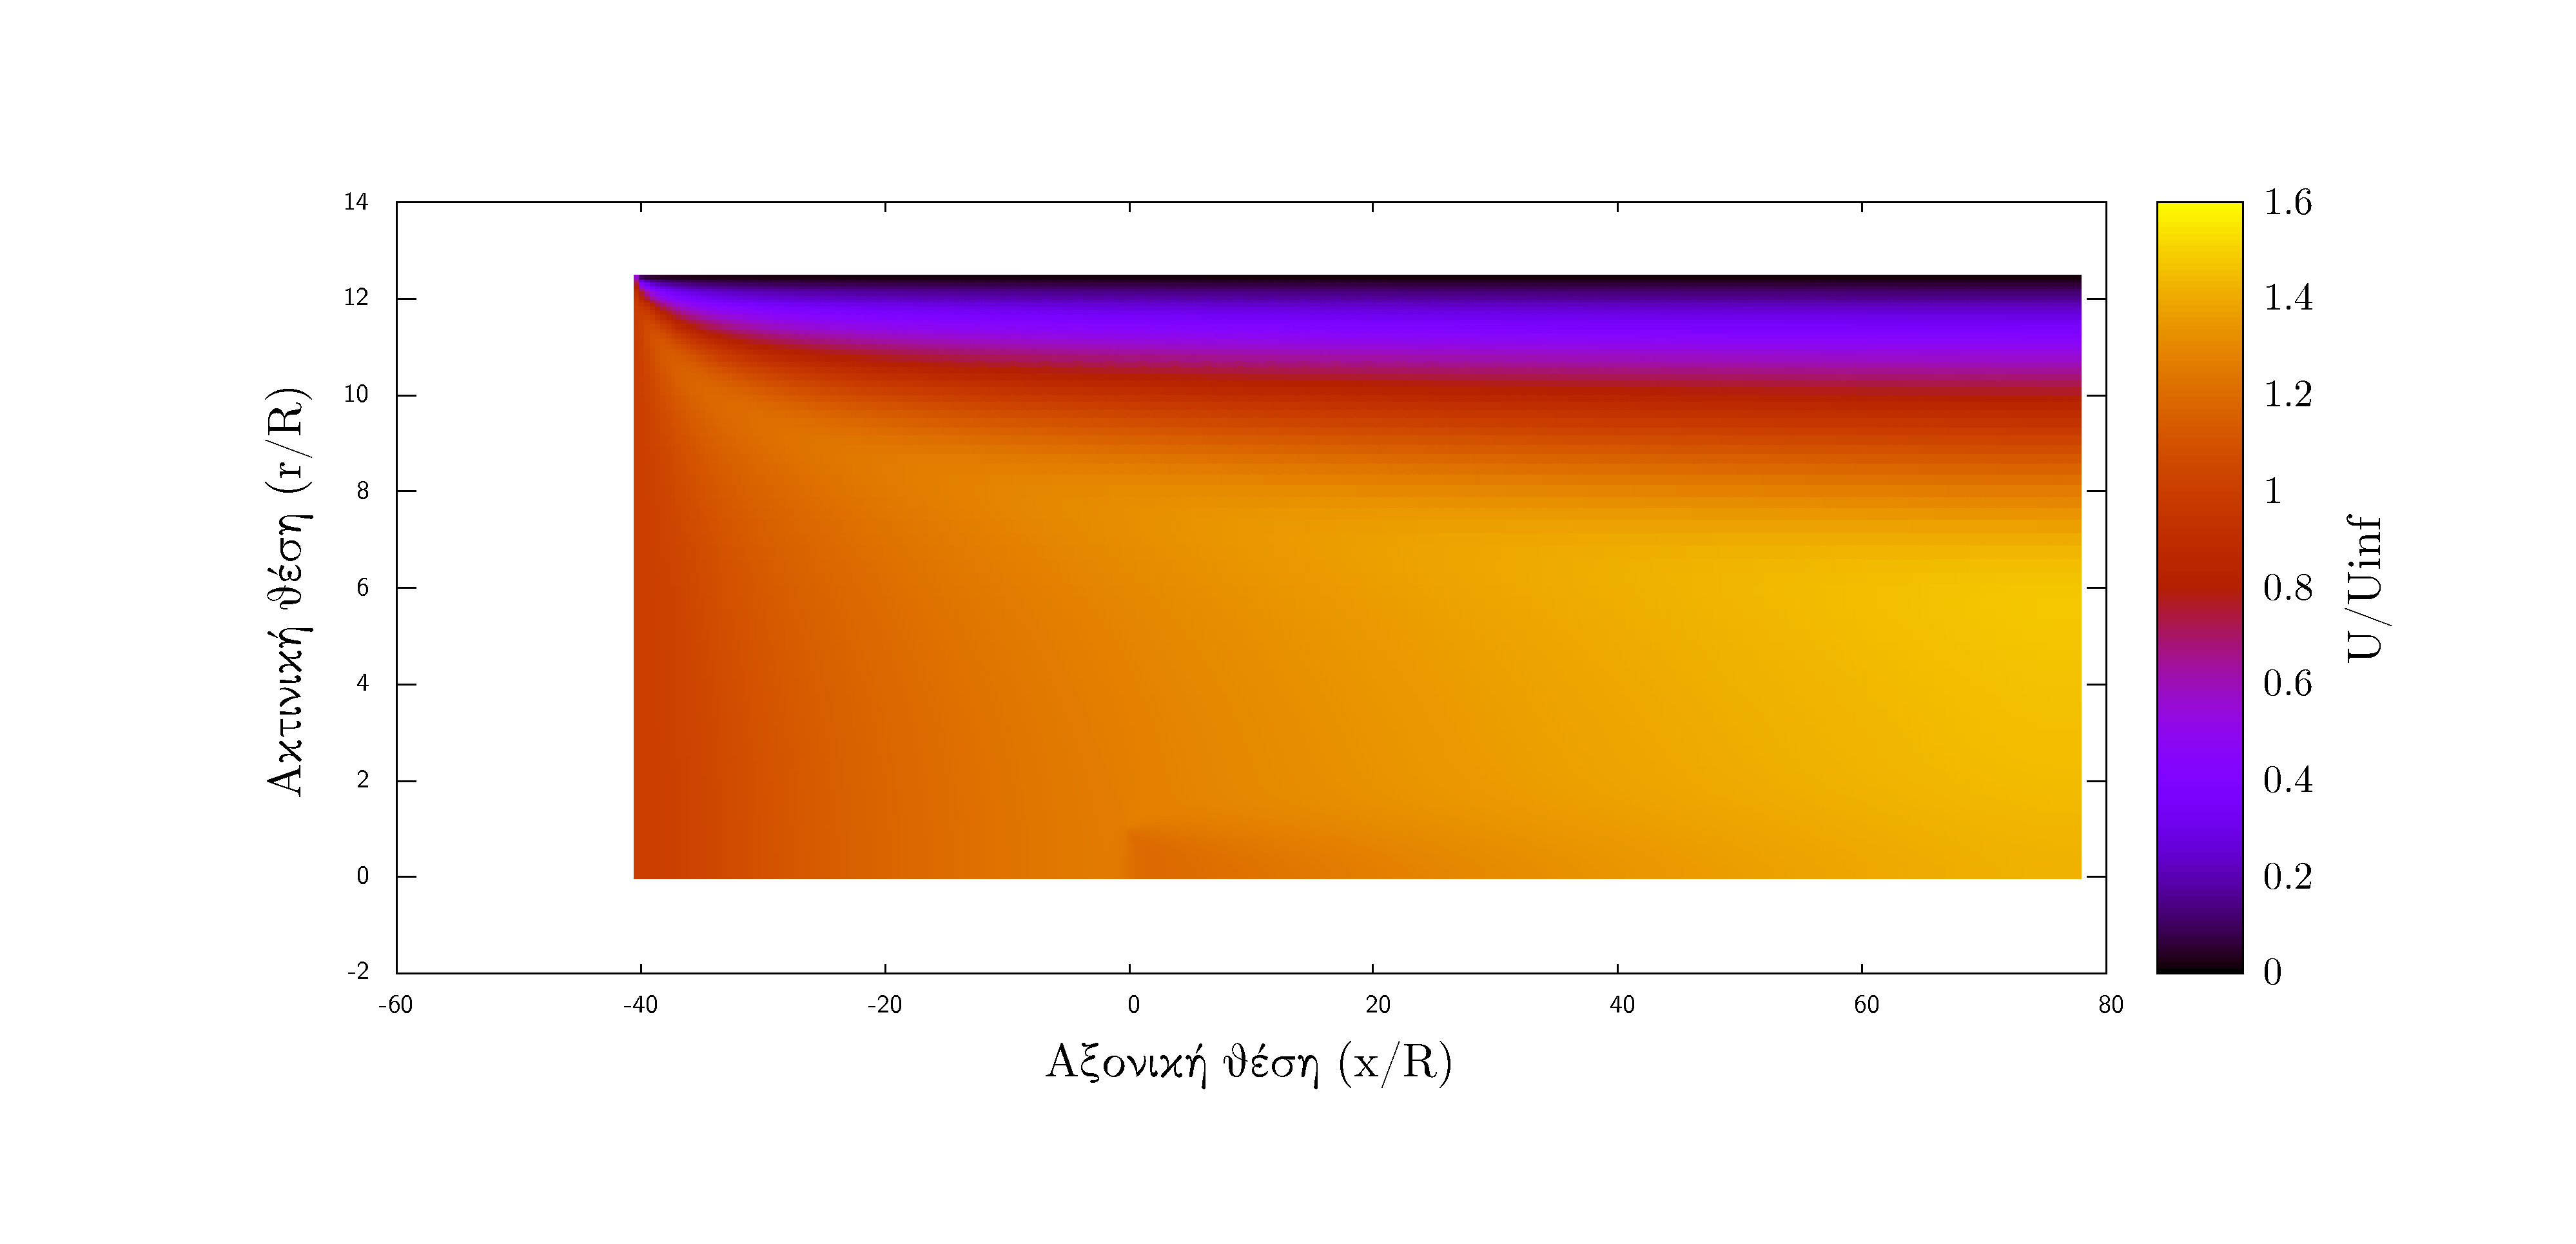
\includegraphics[width=0.85\textwidth]{figures/isoU.pdf}
    \end{center}
    \caption{Ισοταχείς του πεδίου ροής}
    \label{fig:isoU}
\end{figure}

\begin{figure}[h!]
    \begin{center}
        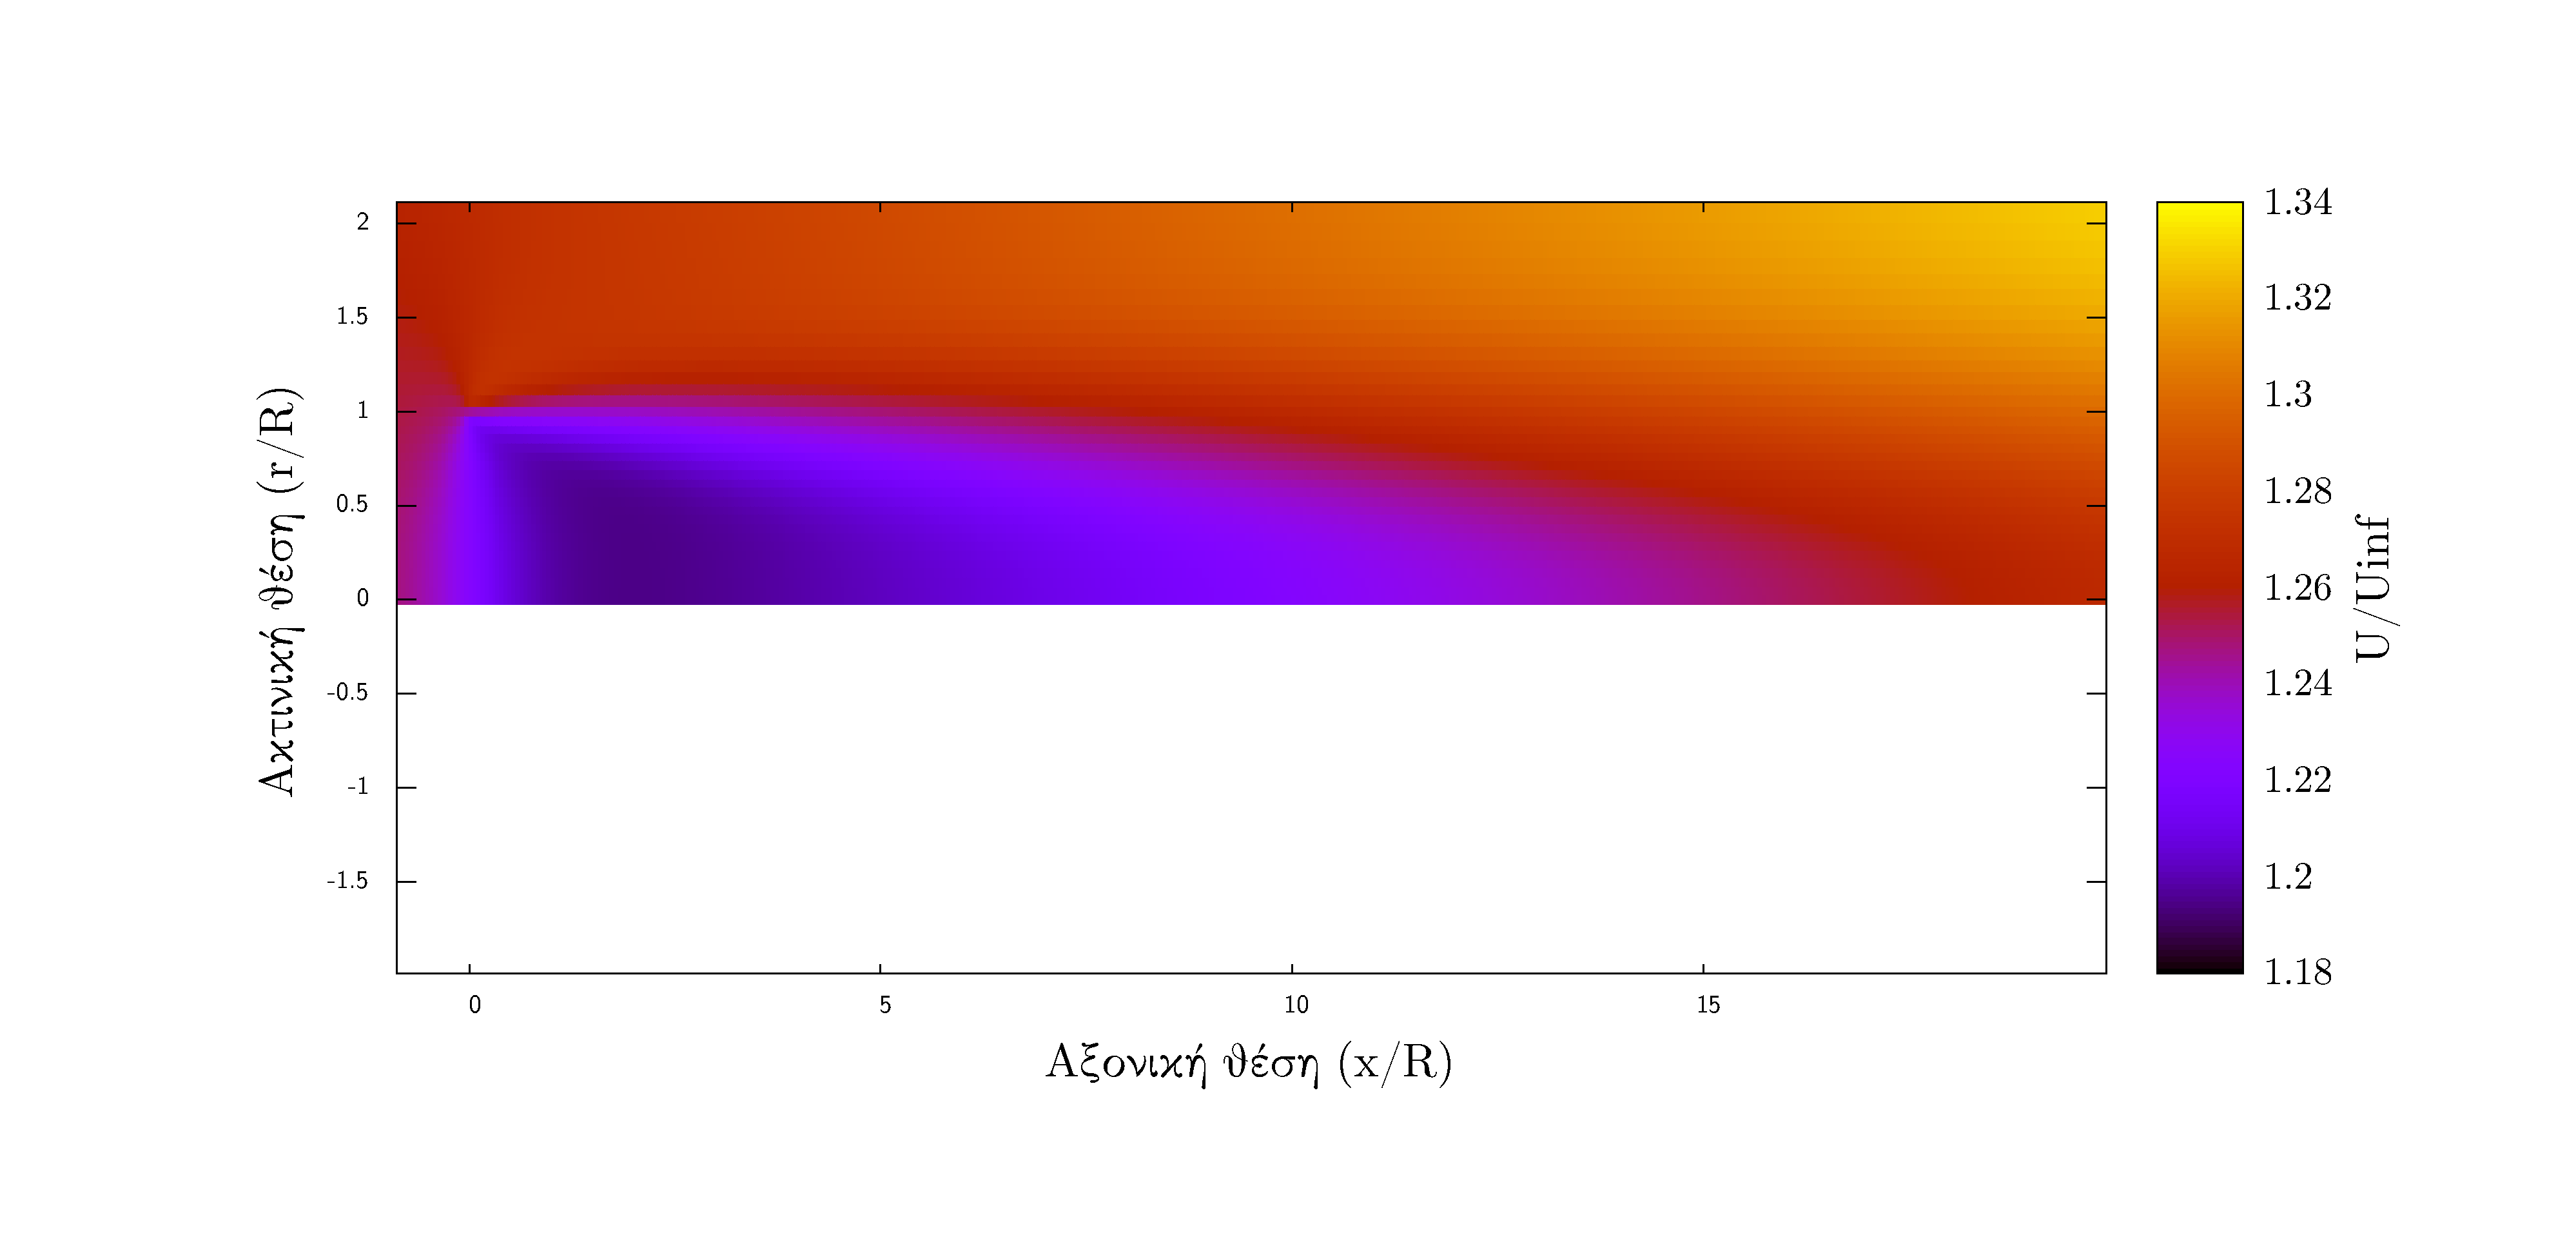
\includegraphics[width=0.85\textwidth]{figures/isoU_zoom.pdf}
    \end{center}
    \caption{Ισοταχείς του πεδίου ροής - μεγέθυνση στην περιοχή του δρομέα}
    \label{fig:isoU_zoom}
\end{figure}


\begin{figure}[h!]
    \centering
    \subfigure[]{%
        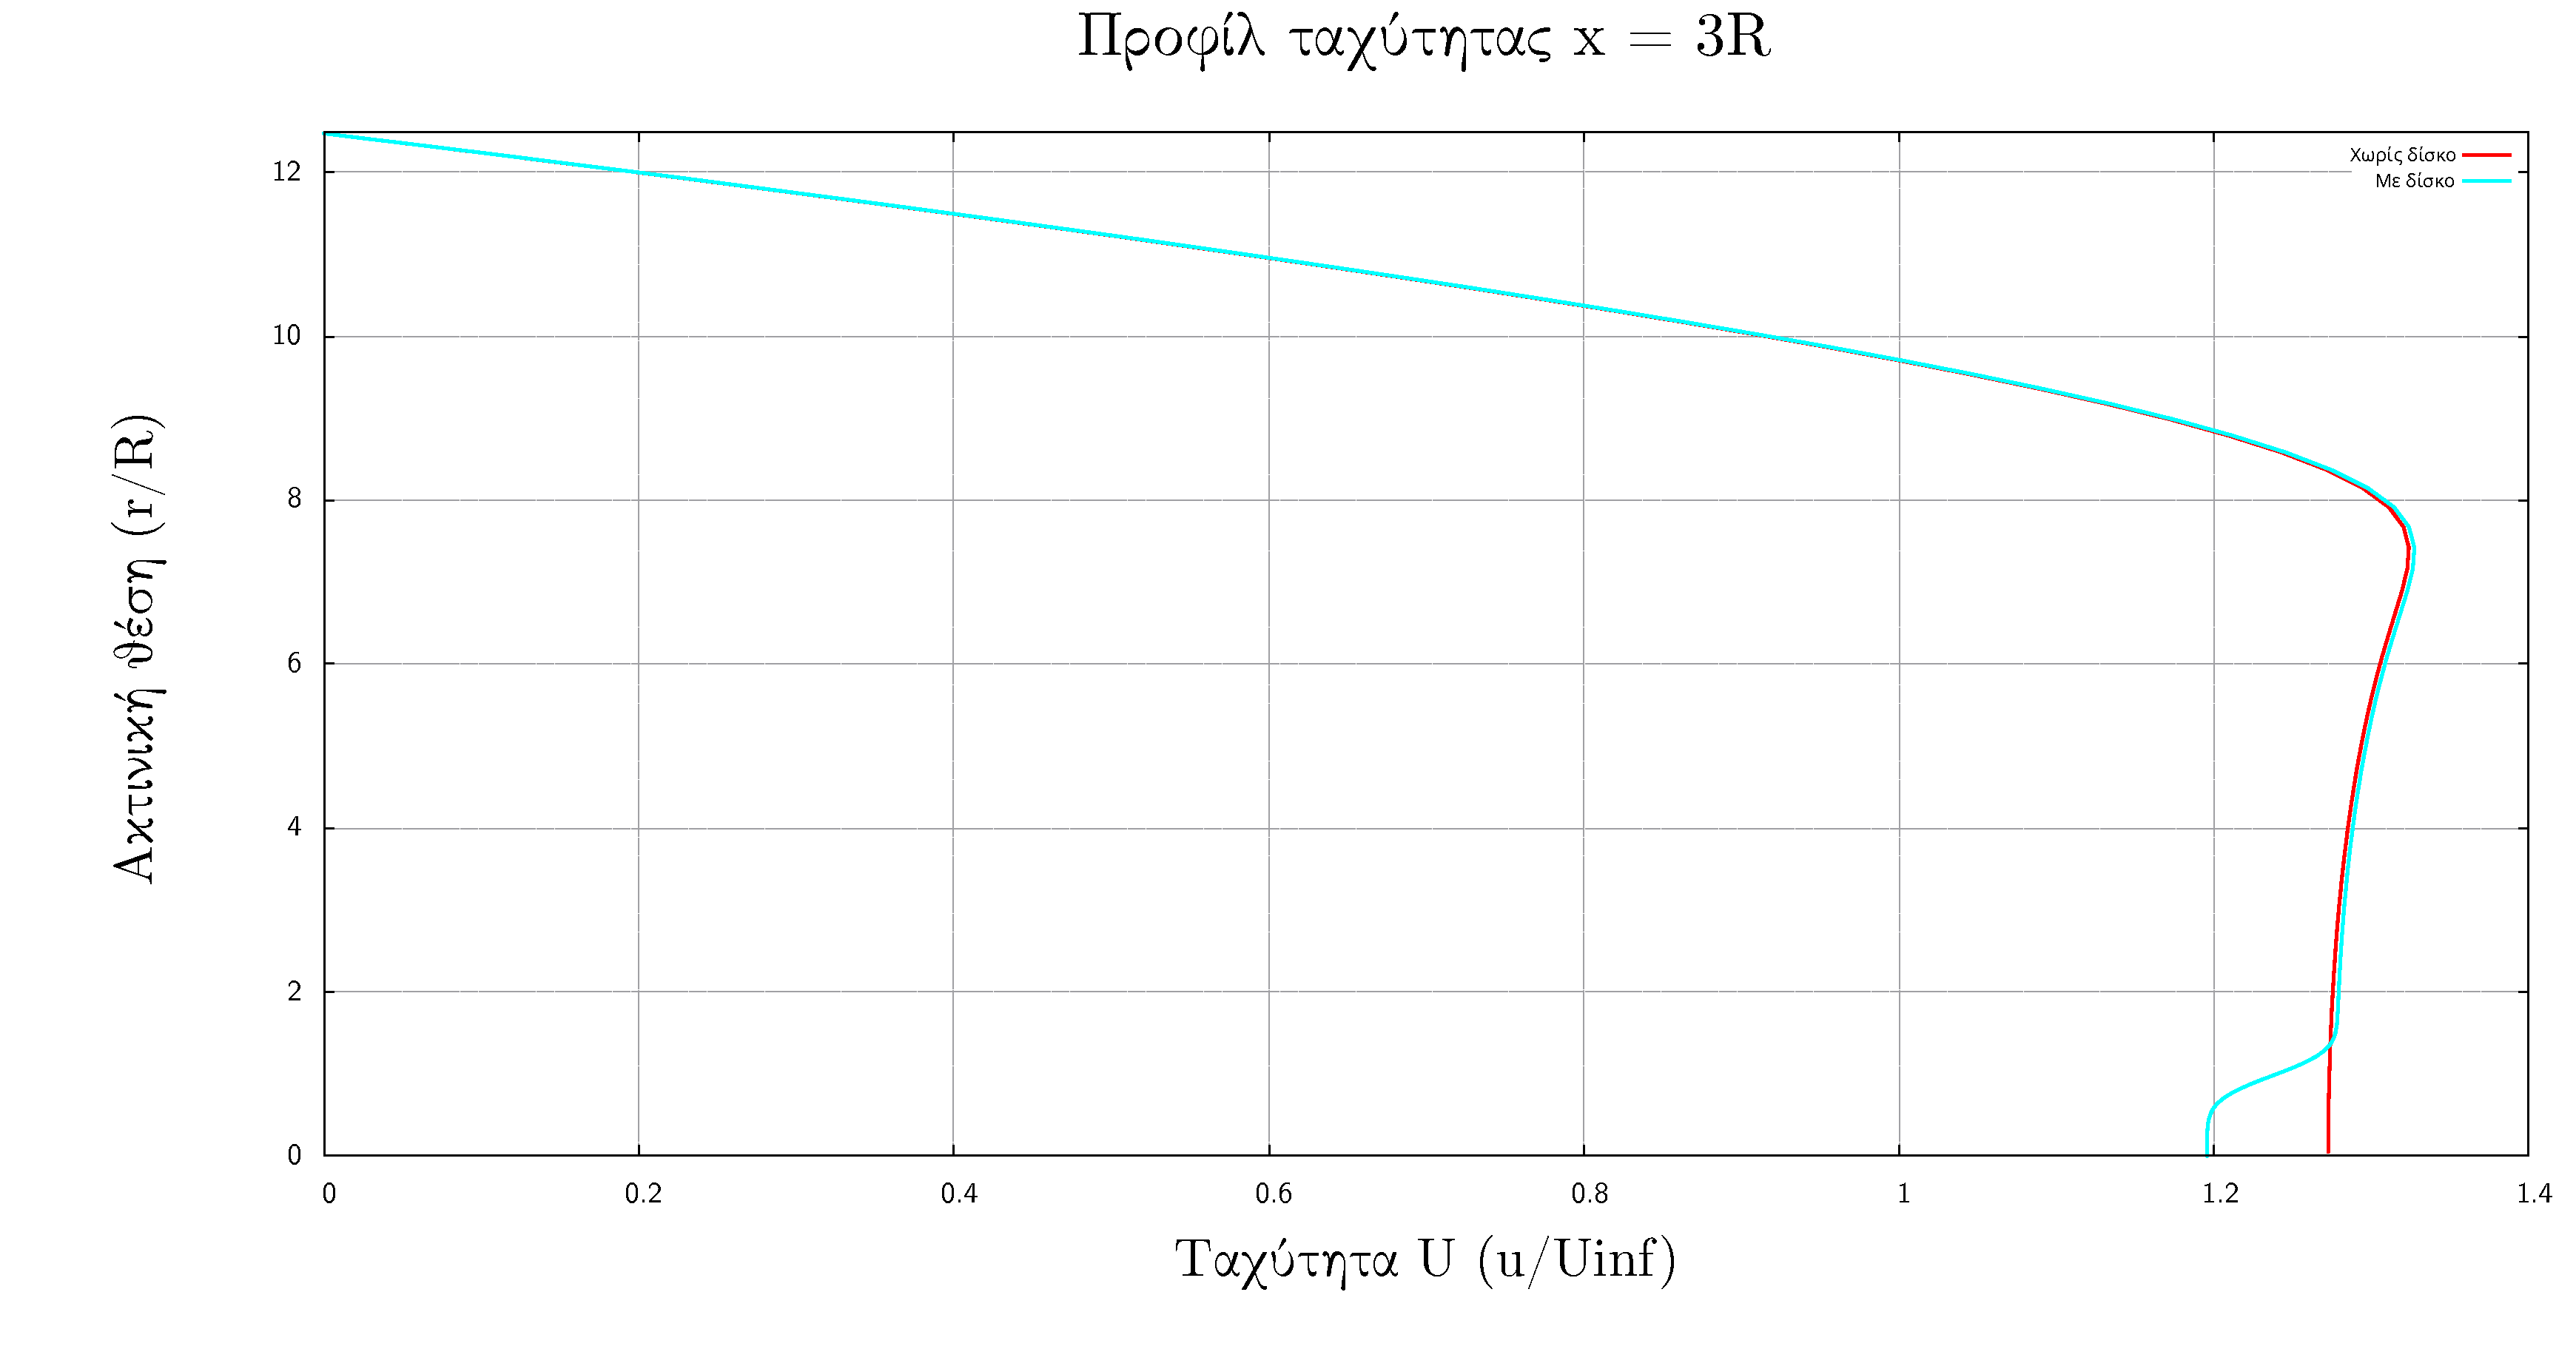
\includegraphics[width=0.3\textwidth]{figures/x3/x3_u.pdf}%
        \caption{Plot 1}%
        \label{fig:plot1}}
    \hfill
    \subfigure[]{%
        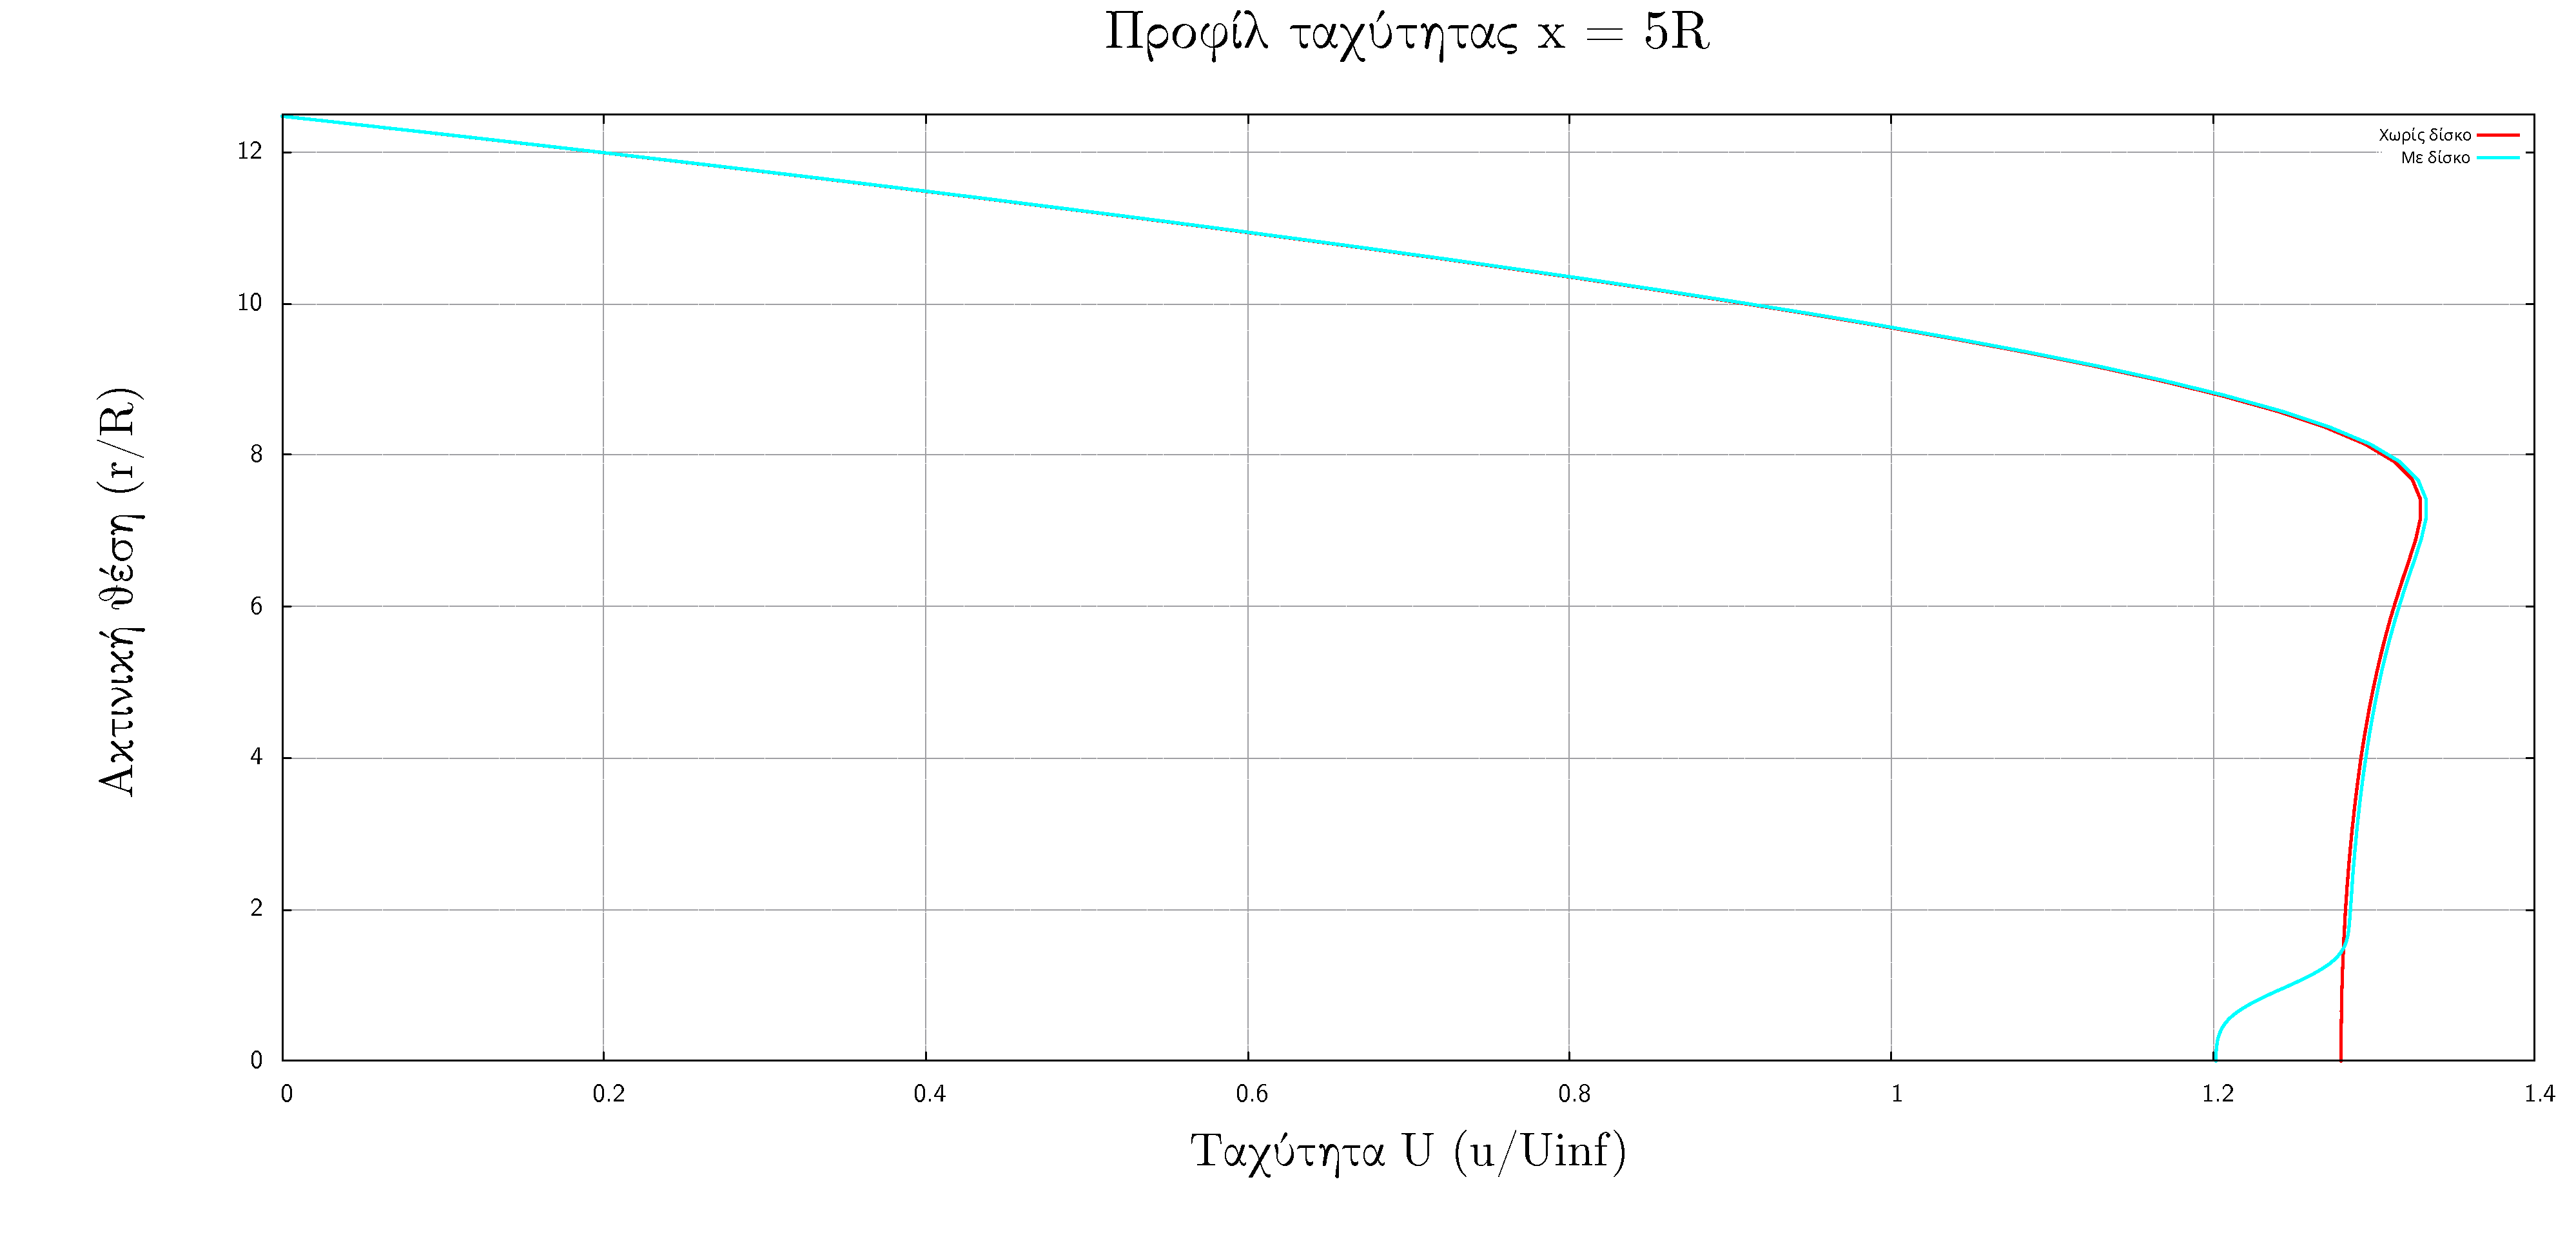
\includegraphics[width=0.3\textwidth]{figures/x5/x5_u.pdf}%
        \caption{Plot 2}%
        \label{fig:plot2}}
    \hfill
    \subfigure[]{%
        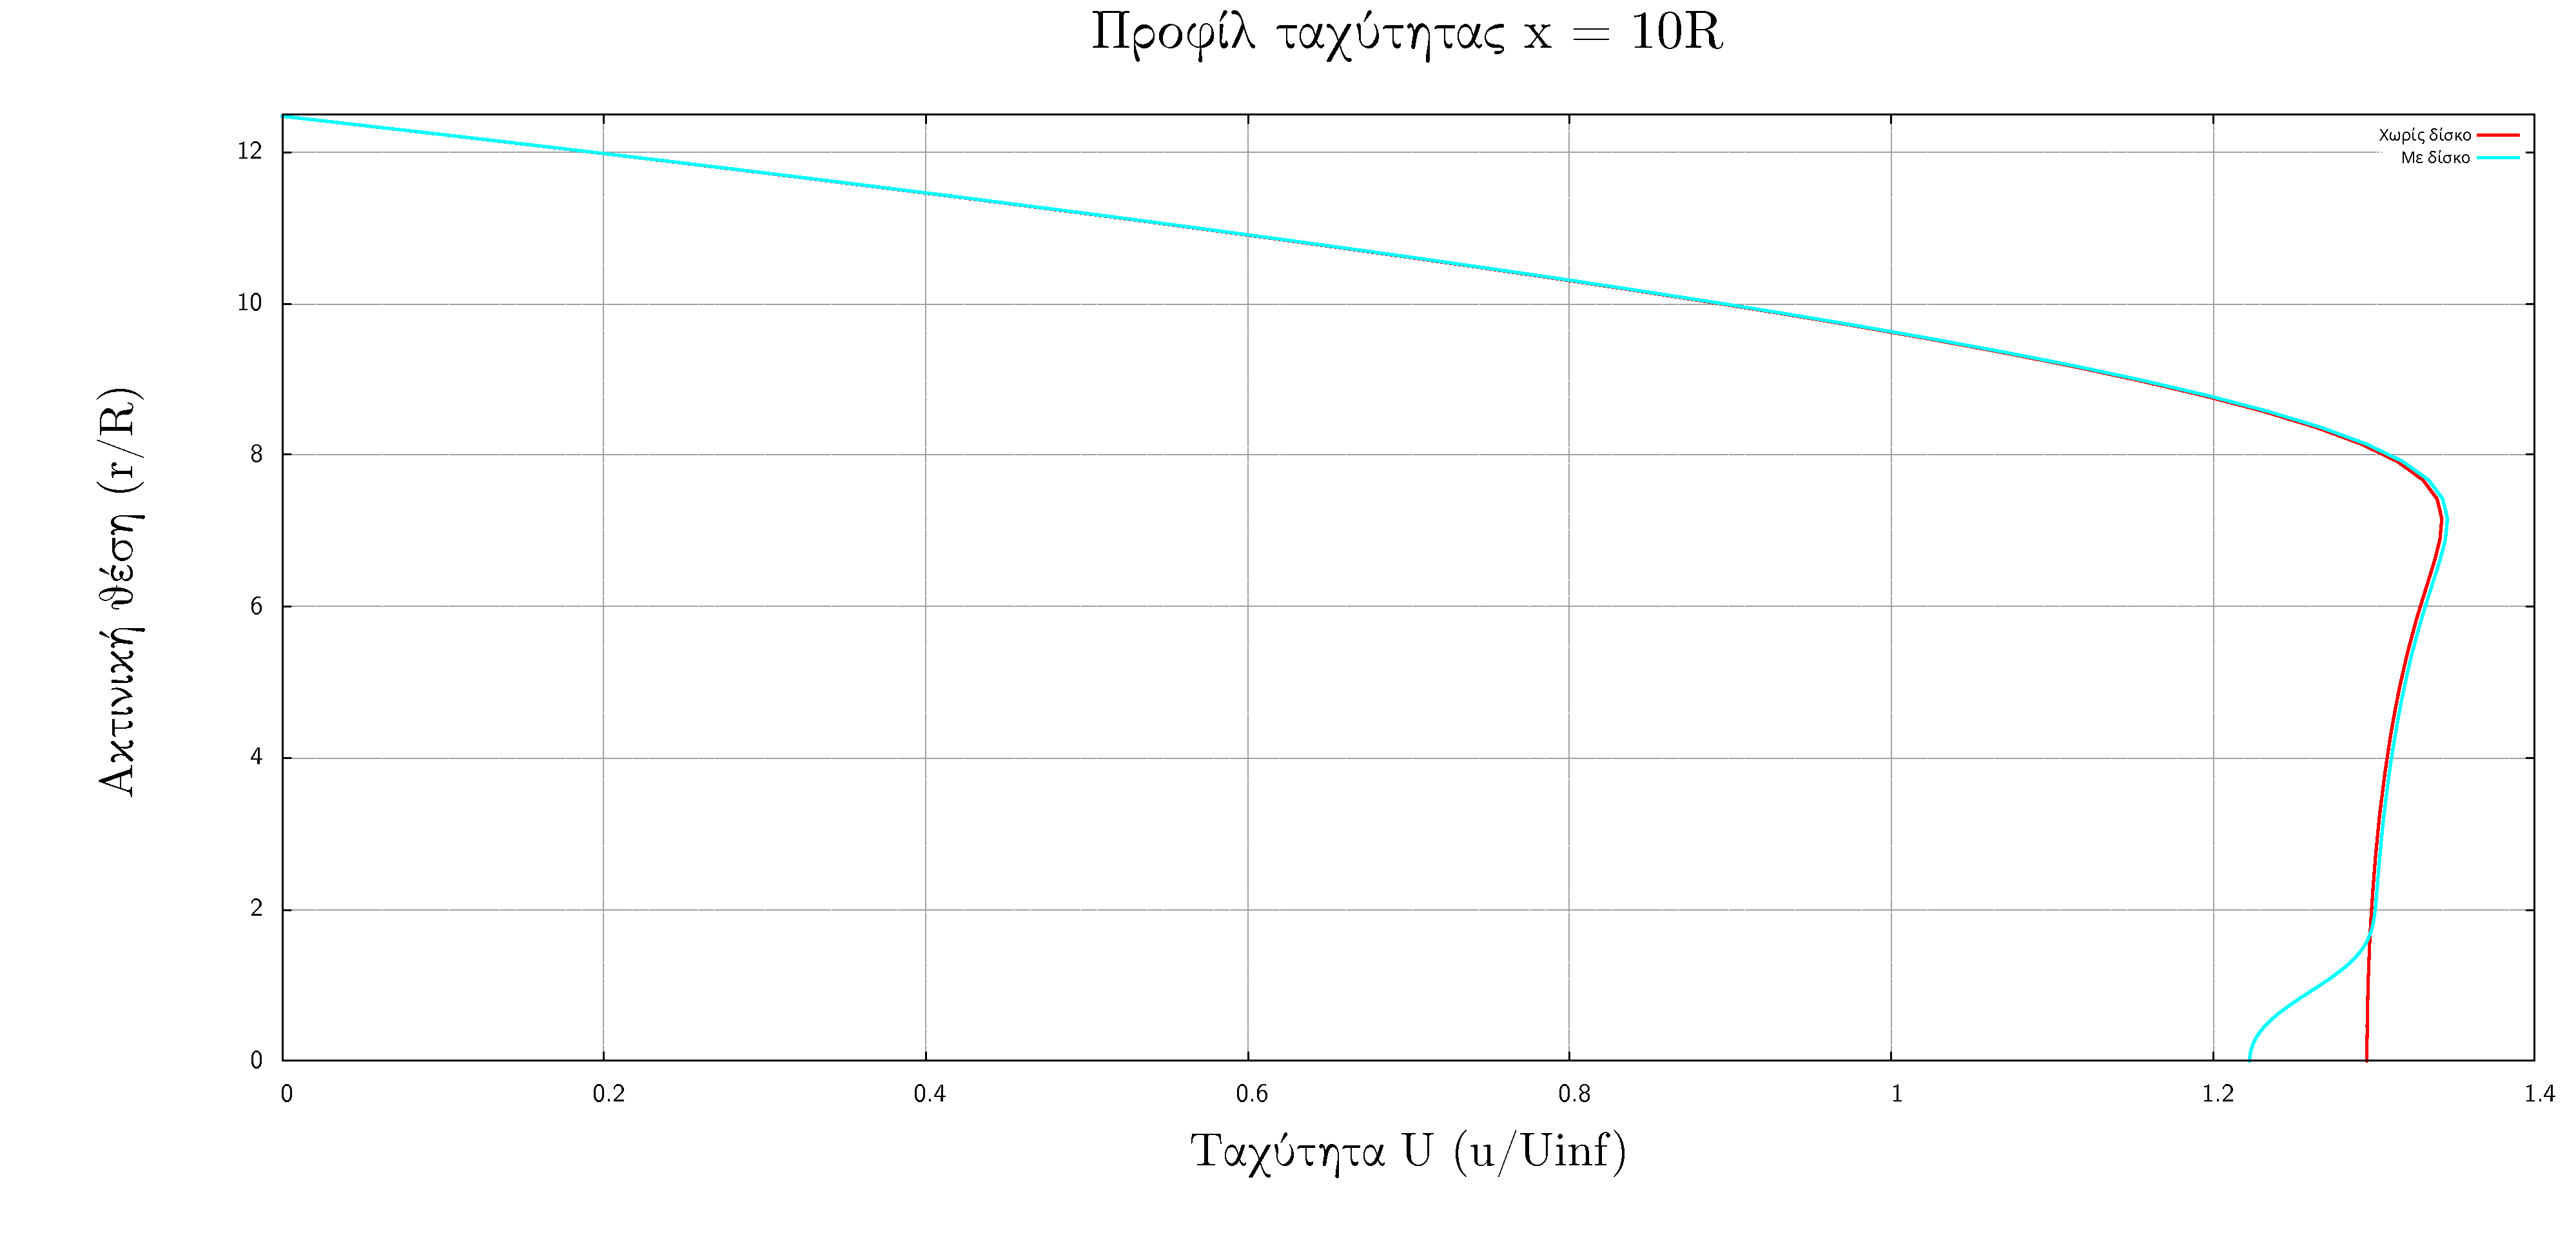
\includegraphics[width=0.3\textwidth]{figures/x10/x10_u.pdf}%
        \caption{Plot 3}%
        \label{fig:plot3}}
    
    \medskip
    
    \subfigure[]{%
    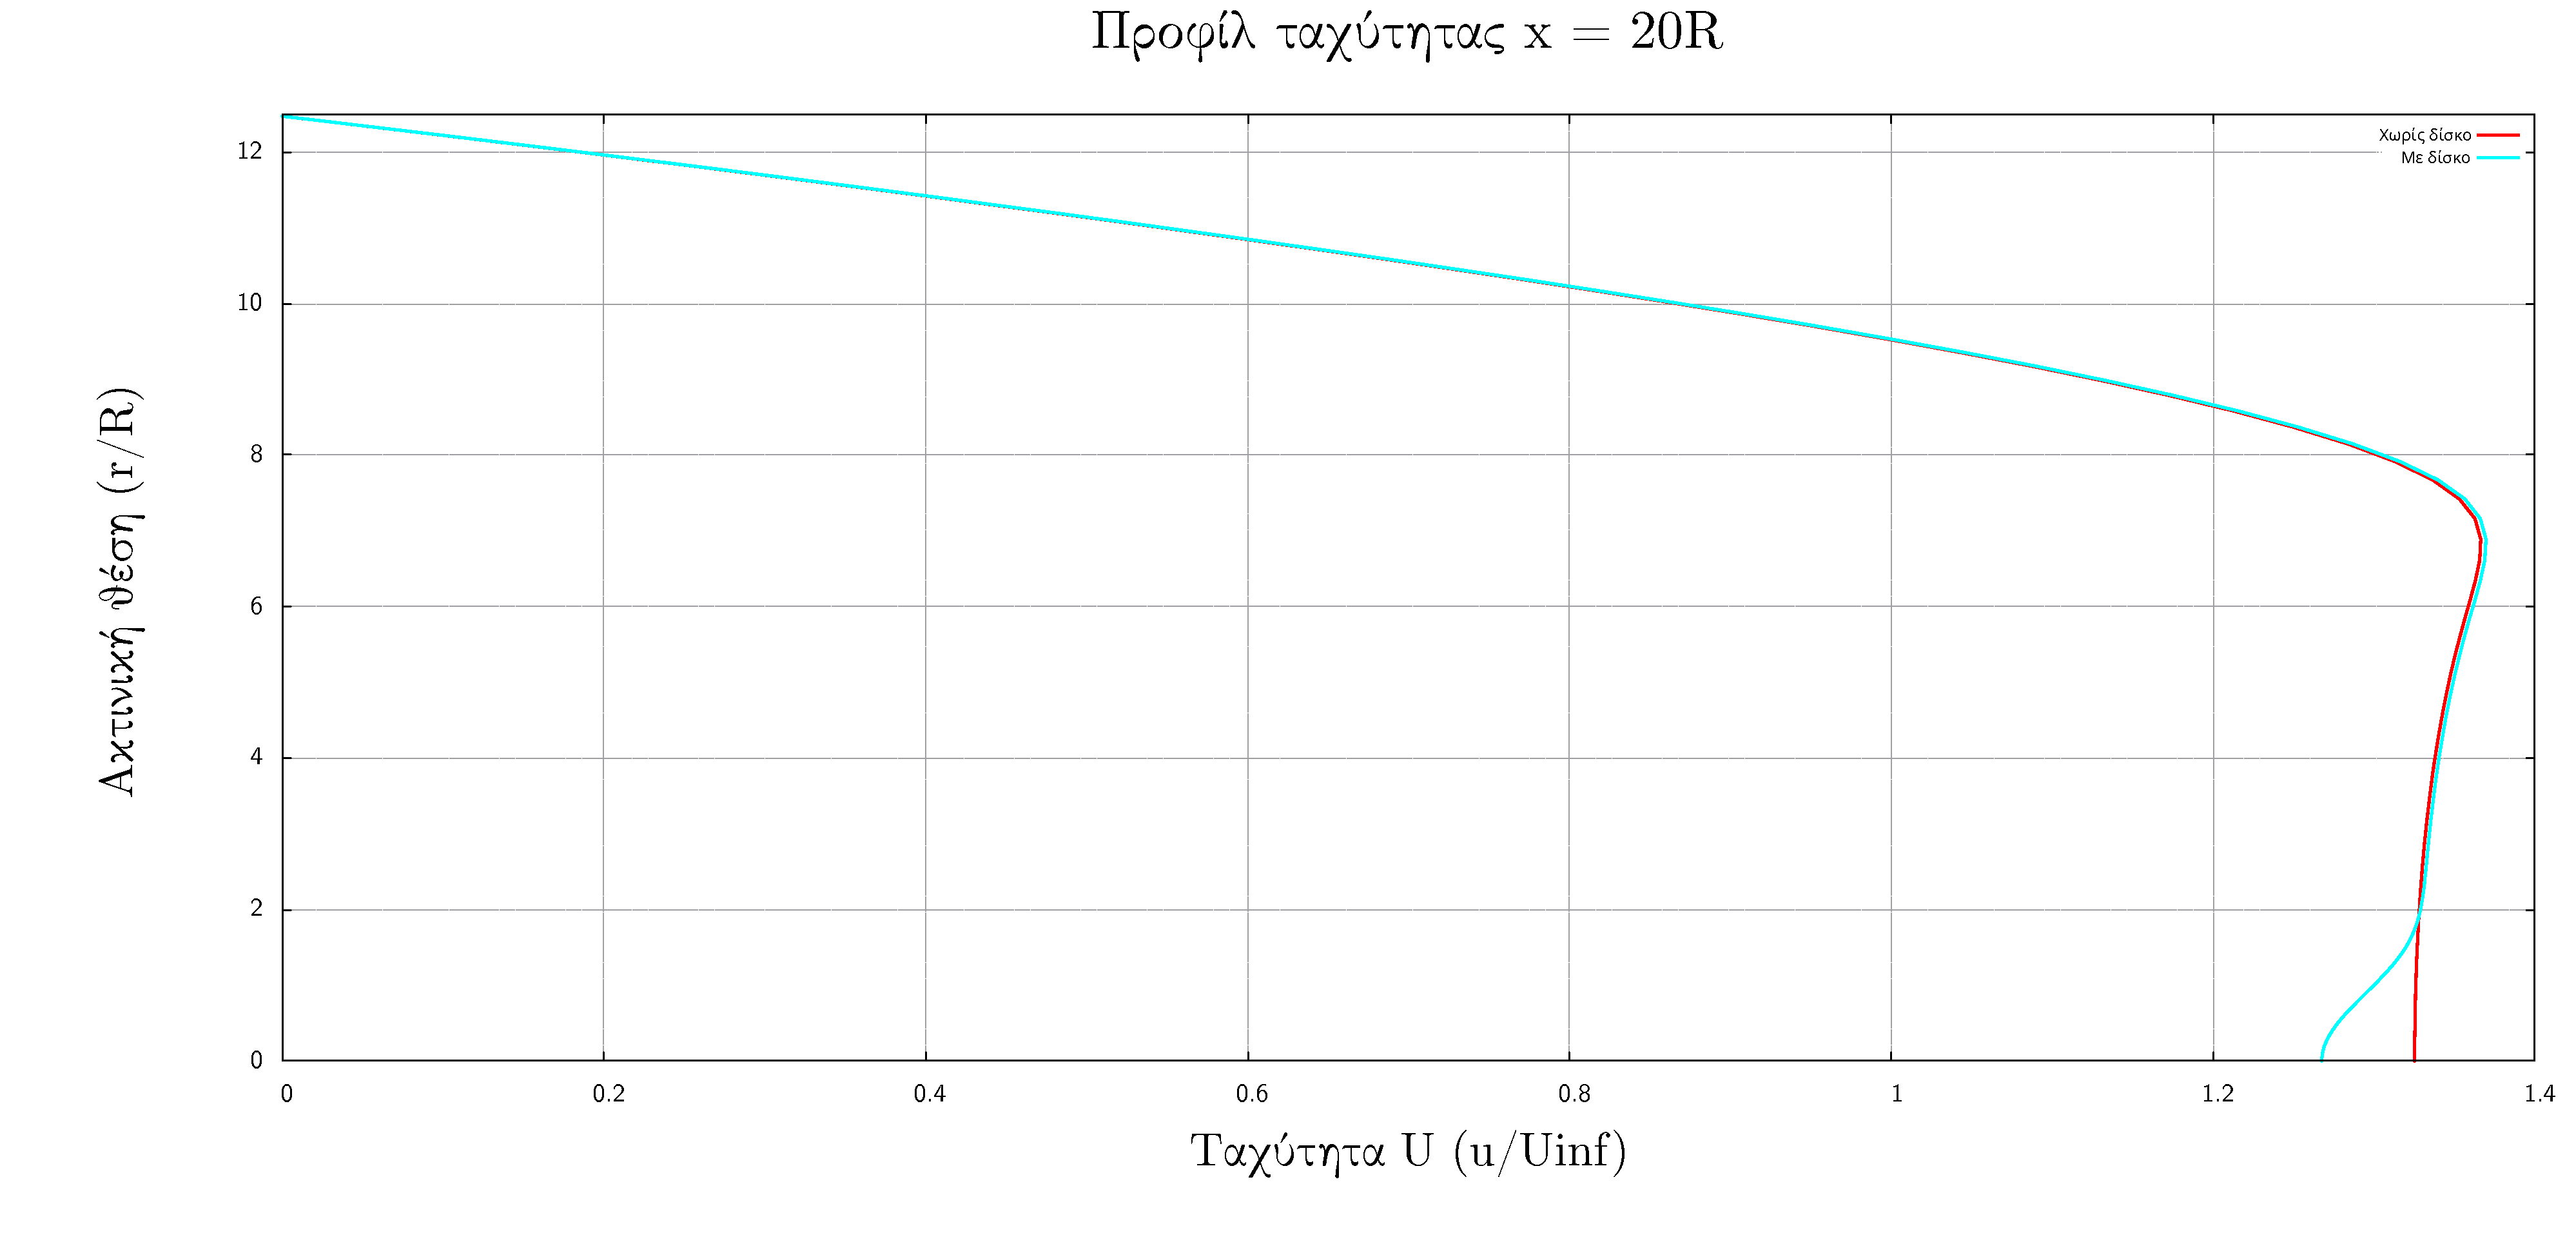
\includegraphics[width=0.5\textwidth]{figures/x20/x20_u.pdf}%
        \caption{Plot 4}%
        \label{fig:plot4}}
    \hfill
    \subfigure[]{%
        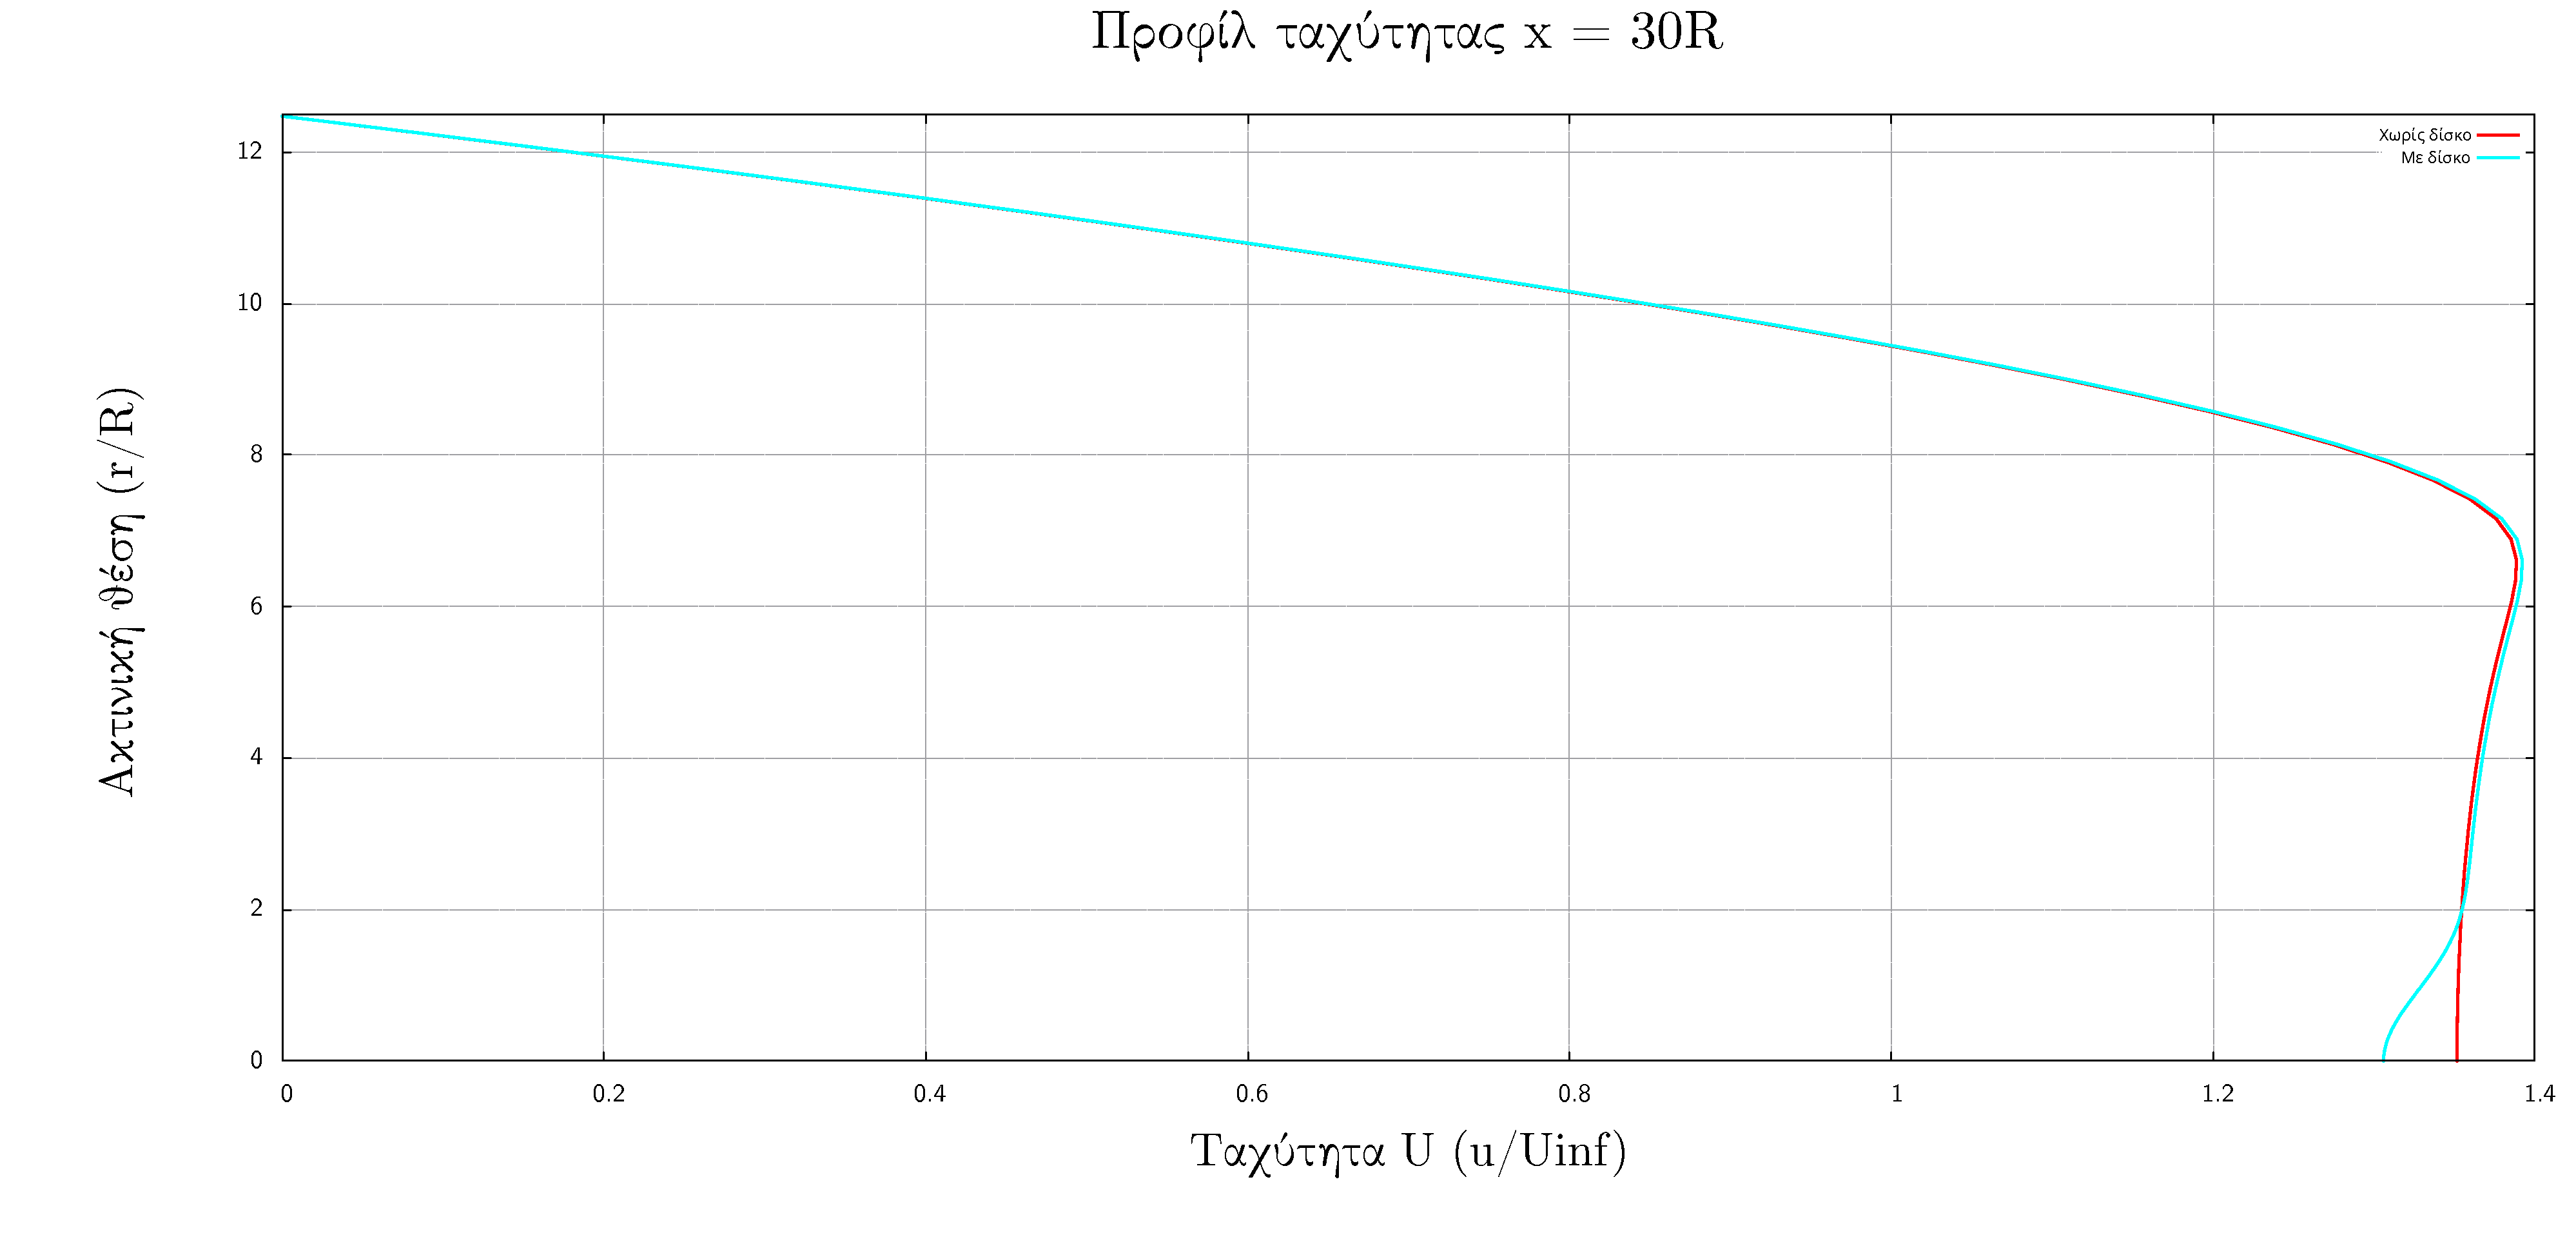
\includegraphics[width=0.5\textwidth]{figures/x30/x30_u.pdf}%
        \caption{Plot 5}%
        \label{fig:plot5}}
    \caption{Collection of Plots}
    \label{fig:all_plots}
\end{figure}

%
%\begin{figure}[h!]%
%\centering
%\subfigure[]{%
%\label{fig:first}%
%\includegraphics[width = 0.45\textwidth]{Graphs/theor_mo.jpg}}%
%\qquad
%\subfigure[]{%
%\label{fig:second}%
%\includegraphics[width = 0.45\textwidth]{Graphs/act_mo.jpg}}%
%\caption{(α): Θεωρητική μηνιαία παραγωγή ενέργειας, (β) Πραγματική μηνιαία παραγωγή ενέργειας}
%\label{fig:month}
%\end{figure}
